\documentclass[11pt]{article}
\usepackage[a4paper, portrait, margin=1in]{geometry}
\usepackage{hyperref}
\usepackage{graphicx}

\newcommand{\myname}{Tom Sydney Kerckhove}
\newcommand{\mynetzh}{tomk}
\newcommand{\myleginr}{15-908-064}

\newcommand{\javafile}[1]{\footnote{\url{https://gitlab.inf.ethz.ch/\mynetzh/asl-fall16-project/blob/master/asl/src/ch/ethz/asl/#1.java}}}
\newcommand{\plot}[1]{plots/#1}
\newcommand{\asset}[1]{assets/#1}


\newcommand{\java}[1]{\mintinline{java}{#1}}


\begin{document}

\title{Advanced Systems Lab (Fall'16) -- First
Milestone}

\author{\textbf{Name: \emph{\myname}}\\\textbf{Legi number: \emph{\myleginr}}}

\date{
\vspace{4cm}
\textbf{Grading} \\
\begin{tabular}{|c|c|}
\hline  \textbf{Section} & \textbf{Points} \\
\hline  1.1 &  \\ 
\hline  1.2 &  \\ 
\hline  1.3 &  \\ 
\hline  1.4 &  \\ 
\hline  2.1 &  \\ 
\hline  2.2 &  \\ 
\hline  3.1 &  \\ 
\hline  3.2 &  \\ 
\hline  3.3 &  \\ 
\hline \hline Total & \\
\hline 
\end{tabular} 
}

\maketitle
\newpage

\section{System Description}\label{sec:system-description}

\subsection{Overall Architecture}\label{sec:desc:architecture}



\subsection{Load Balancing and Hashing}\label{sec:desc:hashing}


\subsection{Write Operations and Replication}\label{sec:desc:writes}


\subsection{Read Operations and Thread Pool}\label{sec:desc:reads}



\section{Memcached Baselines}\label{sec:baseline}


\subsection{Throughput}\label{sec:baseline:tput}

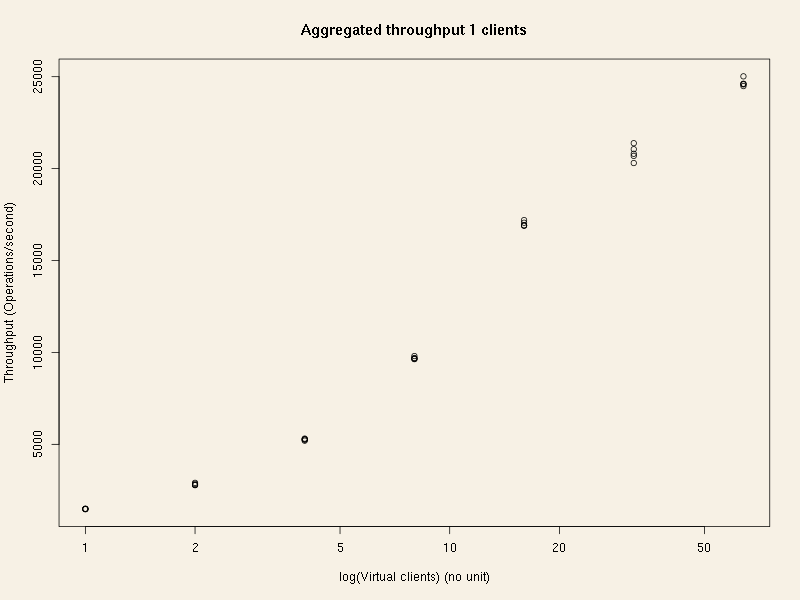
\includegraphics[width=0.5\textwidth]{../analysis/remote-baseline-experiment-tps-1.png}
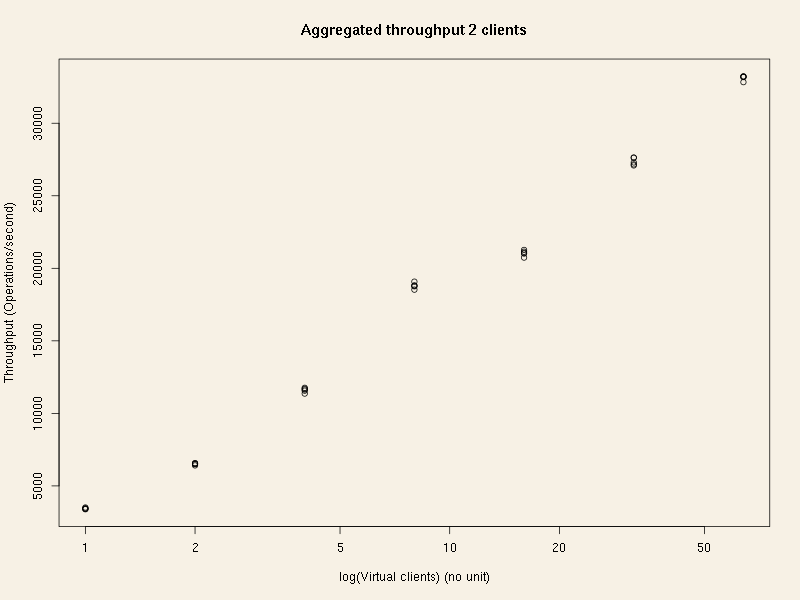
\includegraphics[width=0.5\textwidth]{../analysis/remote-baseline-experiment-tps-2.png}

\subsection{Response time}\label{sec:baseline:rt}

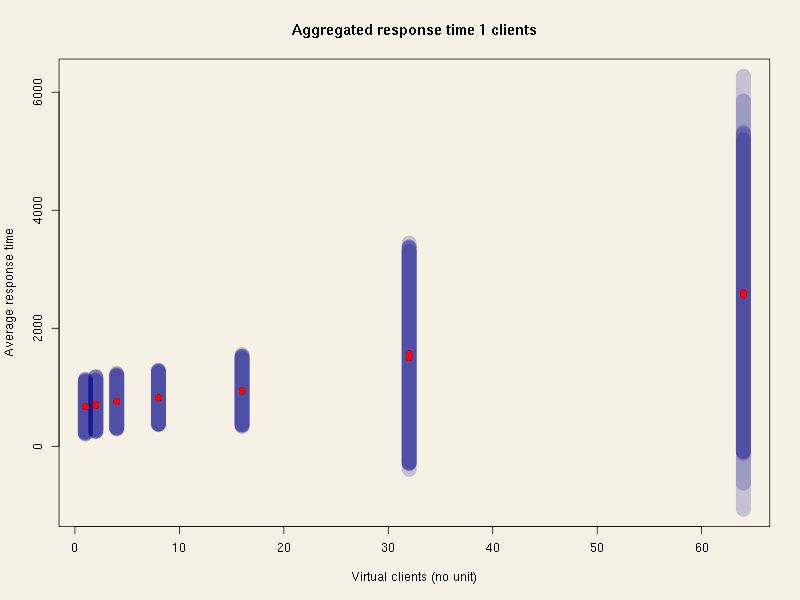
\includegraphics[width=0.5\textwidth]{../analysis/remote-baseline-experiment-avg-1.png}
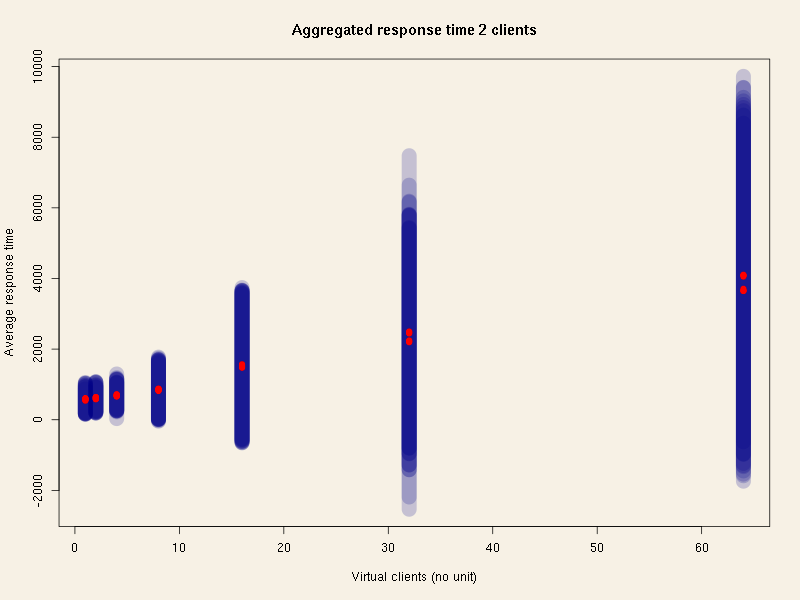
\includegraphics[width=0.5\textwidth]{../analysis/remote-baseline-experiment-avg-2.png}
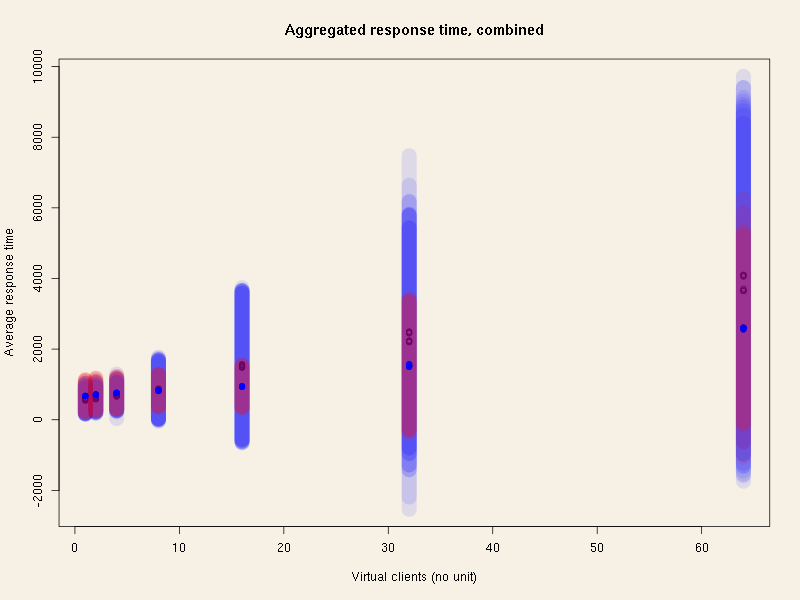
\includegraphics[width=0.5\textwidth]{../analysis/remote-baseline-experiment-avg-combined.png}

\section{Stability Trace}\label{sec:trace}


\subsection{Throughput}

\subsection{Response time}

\subsection{Overhead of middleware}



\pagebreak

\section*{Logfile listing}



\end{document}
